% Monte Carlo tree search (MCTS) 4-stage diagram: selection, expansion, rollout, and backpropagation.
\tikzset{
    nodes={draw, circle}, >=latex, -, level distance=0.5in,
    every node/.style={draw=black, thin, minimum size=6mm},
    norm/.style={edge from parent/.style={black,thin,draw}},
    emph1/.style={edge from parent/.style={line width=1.6pt,draw}},
    emph2/.style={edge from parent/.style={line width=2.0pt,draw}},
    emph3/.style={edge from parent/.style={line width=2.4pt,draw}},
    emph4/.style={edge from parent/.style={line width=1.6pt,draw}}, % rollout
    semiselected/.style={line width=1.6pt},
    selected/.style={line width=1.6pt},
    root/.style={label=\textsc{#1}},
    baseline=(selection-root.base),
    state/.style={circle, norm,-},
    action/.style={rectangle, norm},
    rollout-end/.style={rectangle, draw=none, minimum height=0mm},
    rollout-edge/.style={->, decorate, decoration={snake, amplitude=1mm, post length=10pt, segment length=12pt}, dotted, line cap=round, dash pattern=on 0pt off 2\pgflinewidth},
}
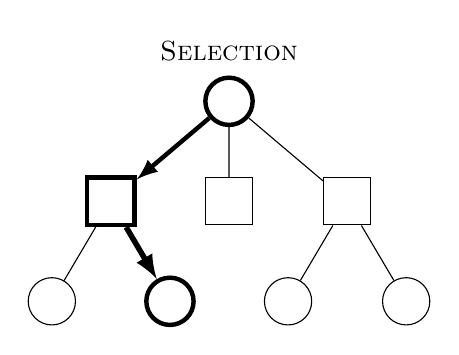
\begin{tikzpicture}
    \node [root=Selection, state, selected] (selection-root) {}
        child [emph1, ->] { node [action, selected] {}
            child [state] { node {} }
            child [state, emph2, ->] { node [selected] {} }
        }
        child [state] {node [action] {}}
        child [state] {node [action] {}
            child [state] { node {} }
            child [state] { node {} }
        };
\end{tikzpicture}
\hspace{1cm}
\begin{tikzpicture}
    \node [root=Expansion, state] {}
        child { node [action] {}
            child [state] { node {} }
            child [state] { node [semiselected] {}
                child [state, emph3] { node [action, selected] {} }
            }
        }
        child [state] {node [action] {}}
        child [state] {node [action] {}
            child [state] { node {} }
            child [state] { node {} }
        };
\end{tikzpicture}
\hspace{1cm}
\begin{tikzpicture}
    \node [root=Rollout, state] {}
        child { node [action] {}
            child [state] { node {} }
            child [state] { node {}
                child [state] { node [action, selected] {}
                    child [state, emph4, level distance=0.74in] { node [rollout-end] {$Q$}
                        edge from parent [rollout-edge]
                    }
                }
            }
        }
        child [state] {node [action] {}}
        child [state] {node [action] {}
            child [state] { node {} }
            child [state] { node {} }
        };
\end{tikzpicture}
\hspace{1cm}
\begin{tikzpicture}
    \node [root=Backpropagation, state, selected] {}
        child [<-,emph1] { node [action, selected] {}
            child [state] { node {} }
            child [state, emph2, <-] { node [selected] {}
                child [state, emph3, <-] { node [action, selected] {$Q$} }
            }
        }
        child [state] {node [action] {}}
        child [state] {node [action] {}
            child [state] { node {} }
            child [state] { node {} }
        };
\end{tikzpicture}
